\documentclass[12pt]{article}
\usepackage[utf8]{inputenc}
\usepackage[russian]{babel}
\usepackage{graphicx}
\usepackage{wrapfig}
\usepackage{hyperref}
\usepackage{epsf,amsmath,amsfonts,amssymb,amsbsy}
\usepackage[mathscr]{eucal}
\usepackage[left=1.5cm,right=1.5cm,
    top=2cm,bottom=2cm,bindingoffset=0cm]{geometry}
\usepackage{cmlgc}
\usepackage{array}
\usepackage{wrapfig}
\usepackage{lipsum}
\usepackage{esvect}
\usepackage{subfig}
\usepackage{calc}
\usepackage{pgfplots,tikz,circuitikz}
\usepackage{pgfplotstable}
\usepackage{tkz-euclide}

\usepackage{centernot}
\usepackage{cancel}

%Includes "References" in the table of contents
\usepackage[nottoc]{tocbibind}

\usepackage{csvsimple}


\begin{filecontents*}{data.csv}
\end{filecontents*}

\title{3.4.2}
\author{panferov.ad }
\date{September 2020}

\begin{document}

\begin{center}
  \LARGE{Работа 3.4.5}\\[0.2cm]
  \LARGE{Петля гистерезиса (динамический метод)}\\[0.2cm]
  \large{Панферов Андрей}\\[0.2cm]
\end{center}

\section{Экспериментальная установка}
\textbf{В работе используются:} понижающий трансформатор, реостат, резистор, интегрируюшая цепочка, амперметр и вольтметр (мультиметры), электронный осциллограф, делитель напряжения, переключатель, тороидальные образцы с двумя обмотками.

\textbf{Экспериментальная установка}: Схема установки приведена на рис. \ref{pic1}. Напряжение сети $(220 \mathrm{B}, 50$Гц$)$ через разделительный понижаюший трансформатор Тр подаётся на реостат $R_{1},$ ВКлючённый как потенциометр. Регулируемое напряжение $\sim 6,3$ В подведено к средним точкам переключателя $\mathrm{K}_{0}:$ в положении "$\Pi$" (петля) напряжение подводится к клеммам "$6,3$" на панели установки, В положении "Д" (делитель) - к клеммам делителя напряжения.

С клемм "$6,3$" регулируемое напряжение подаётся на намагничивающуую обмотку $N_{0}$ исследуемого образца.

\begin{center}
    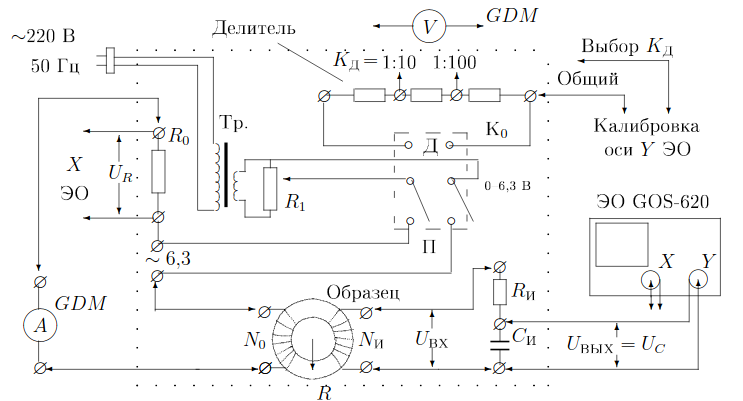
\includegraphics[width=0.8\textwidth]{1.png}
    \label{pic1}
\end{center}

Ток в обмотке $N_{0}$ измеряется мультиметром А. Напряжение с сопротивления $R_{0},$ включенного последовательно с обмоткой $N_{0},$ подаётся на вход $X$ электронного осциллографа (ЭО). Это напряжение пропорционально току в обмотке $N_{0},$ а следовательно и напряжённости $H$ магнитного поля в образце.

Для измерения магнитной индукции $B$ с измерительной обмотки $N_{\text {И }}$ на вход интегрируюшей $R C$ -цепочки подаётся напряжение $U_{\mathrm{BX}},$ пропорциональное производной $\dot{B},$ a $\mathrm{c}$ выхода снимается напряжение $U_{\mathrm{BbIX}}=U_{C},$ пропорциональное величине $B,$ и подаётся на вход $Y$.

Замкнутая кривая, возникающая на экране, воспроизводит в некотором масштабе (различном для осей $X$ и $Y)$ петлю гистерезиса. Чтобы придать этой кривой количественный смысл, необходимо установить масштабы изображения, т.е. провести калибровку каналов $X$ и $Y$ ЭО. Для этого, во-первых, надо узнать, каким напряжениям (или токам) соответствуют амплитуды сигналов, видимых на экране, и во-вторых, - каким значениям $B$ и $H$ соответствуют эти напряжения (или току).

Измерение напряжения с помошью осциллографа. Исследуемый сигнал подаётся на вход $X$ ЭО; длина $2 x$ горизонтальной черты, наблюдаемой на экране, характеризует удвоенную амплитуду сигнала.

Если известна чувствительность усилителя $K_{X}$ в вольтах на деление нгкалы экрана $(\mathrm{B} / \mathrm{cM}),$ то удвоенная амплитуда напряжения определяется произведени-
eM
$$
2 U_{X, 0}=2 x \cdot K_{X}
$$
Напряжение, подаваемое на ось $Y,$ измеряется аналогично. Калибровку осей осциллографа $\left(K_{X}\right.$ и $\left.K_{Y}\right)$ можно использовать для построения кривой гистерезиса в координатах $B$ и $H:$

Зная величину сопротивления $R_{0},$ с которого снимается сигнал, можно рассчитать чувствительность канала по току $K_{X I}=K_{X} / R_{0}[\mathrm{A} /$ дел $]$, затем определить цену деления шкалы ЭО в $A / M$
Проверка калибровки горизонтальной оси ЭО с помошью амперметра проводится при закороченной обмотке $N_{0} .$ Эта обмотка с помещённым В неё ферромагнитным образцом является нелинейным элементом, так что ток в ней не имеет синусоидальной формы, и это не позволяет связать амплитуду тока с показаниями амперметра.

При закороченной обмотке $N_{0}$ амперметр А измеряет эффективное значение синусоидального тока $I$эф , текущего через известное сопротивление $R_{0} .$ Сигнал с этого сопротивления подаётся на вход $X$ ЭО. Измерив $2 x$ длину горизонтальной прямой на экране, можно рассчитать $m_{X}$ - чувствительность канала $X:$
$$
m_{X}=2 R_{0} \sqrt{2} I_{\ni \Phi} /(2 x) \quad[\mathrm{B} / \text { Дел }]
$$
Проверка калибровки вертикальной оси ЭО с помошью вольтметра. Сигнал с потенциометра $R_{1}$ подаётся на вход делителя напряжения $\left(\mathrm{K}_{0}\right.$ в положении "Д". Часть этого напряжения снимается с делителя с коэффициентом деления $K_{\text {Д }}(1 / 10$ или $1 / 100)$ и подаётся на вход $Y$ ЭО $($ вместо напряжения $\left.U_{C}\right) .$ Цифровой вольтметр $V$ измеряет напряжение $U_{\text {ЭФ }}$ на этих же клеммах делителя. Измерив $2 y$ - длину вертикальной прямой на экране, можно рассчитать чувствительность канала $Y:$
$$
m_{Y}=2 \sqrt{2} U_{\ni \Phi} /(2 y) \quad[\mathrm{B} / \text { дел }]
$$
При калибровке тороид должен быть отключён, так как несинусои Дальный ток нагрузки в первичной обмотке тороида приводит к искажению формы кривой напряжения и на обмотке трансформатора, питающей делитель.\\
Постоянную времени RС-цепочки можно определить экспериментально. С клемм "6,3" на вход интегрирующей цепочки подаётся синусоидальное напряжение $U_{\mathrm{BX}} .$ На вход $Y$ осциллографа поочерёдно подаются сигналы со входа $\left(U_{\mathrm{BX}}\right)$ и выхода $\left(U_{\mathrm{BHIX}}=U_{C}\right) R C$ -цепочки. Измерив амплитуды этих сигналов с помощью осциллографа, можно рассчитать постоянную времени $\tau=R C .$
$$
R C=\frac{U_{\mathrm{BX}}}{\Omega U_{\mathrm{BBIX}}}
$$

\section{Результаты измерений и их обработка}
\subsection{Калибровка}
\subsubsection{X}
\begin{minipage}{0.6\textwidth}
\begin{center}
\begin{tabular}{|l|l|l|l|l|l|}
\hline
\multicolumn{2}{|l|}{X=20mV}             & \multicolumn{2}{l|}{X=50mV}             & \multicolumn{2}{l|}{X=100mV}             \\ \hline
Дел                & I, mA               & Дел               & I, mA               & Дел                & I, mA               \\ \hline
0                  & 7                   & 0                 & 7                   & 0                  & 7                   \\ \hline
1                  & 35                  & 1                 & 90                  & 1                  & 177                 \\ \hline
2                  & 71                  & 2                 & 174                 & 2                  & 352                 \\ \hline
3                  & 107                 & 3                 & 267                 & 3                  & 537                 \\ \hline
4                  & 144                 & 4                 & 355                 & 4                  & 708                 \\ \hline
5                  & 181                 & 5                 & 443                 & 5                  & 897                 \\ \hline
\multicolumn{2}{|l|}{dI = $50 \pm 3$ mA} & \multicolumn{2}{l|}{dI = $124 \pm 3$ mA} & \multicolumn{2}{l|}{dI = $252 \pm 6$ mA} \\ \hline
\end{tabular}
\label{calX}
\end{center}
\end{minipage}
\begin{minipage}{.4\textwidth}
Откалибруем X канал осциллографа, измерив зависимость показаний последнего от тока через амперметр. Занесем результаты в \textit{Таблицу} \ref{calX}. Рассчитаем коэффециент пересчета делений в ток $dI$ для всех диапазонов.
\end{minipage}
\subsubsection{Y}
\begin{minipage}{0.4\textwidth}
Откалибруем Y канал осциллографа, сравним показания вольтметра и осциллографа и занесем результаты в \textit{Таблицу} \ref{calY}. Домножив U на $2\sqrt{2}$ получим, что в среднем  $U_{vm}$ отличается от $U_{osc}$ на 2\%.
\end{minipage}
\begin{minipage}{0.6\textwidth}
\begin{center}
\begin{tabular}{|l|l|}
\hline
$U_{vm}$, мВ & $U_{osc}$, мВ \\ \hline
20          & 50            \\ \hline
40          & 110           \\ \hline
60          & 170           \\ \hline
80          & 220           \\ \hline
100         & 275           \\ \hline
120         & 325           \\ \hline
140         & 390           \\ \hline
\end{tabular}
\label{calY}
\end{center}
\end{minipage}
\subsection{Феррит}
\begin{minipage}{0.4\textwidth}
\begin{tabular}{|l|l|}
\hline
$N_0$ & 35        \\ \hline
$N_u$ & 400       \\ \hline
$S$   & 3.0см$^2$ \\ \hline
$2\pi R$ & 25см \\ \hline
\end{tabular}
\end{minipage}
\begin{minipage}{0.5\textwidth}
\begin{tabular}{|l|l|l|l|}
\hline
\multicolumn{2}{|l|}{X=50mV} & \multicolumn{2}{l|}{Y=10mV} \\ \hline
$[X_s]$:    & 1.75 дел.    & $217 \pm 18 $mA      &    $30 \pm 3$А/м  \\ \hline
$[Y_s]$:    & 3.75 дел.    & $38 \pm 2$ mV        &   $0.126 \pm 0.007$Тл   \\ \hline
$[X_c]$:    & 0.40 дел.    & $52 \pm 5 $mA        &    $7.2 \pm 0.6$А/м   \\ \hline
$[Y_r]$:    & 1.5 дел.     & $15 \pm 2$mV         &   $0.050 \pm 0.007$Тл   \\ \hline
\end{tabular}
\end{minipage}\\

Измерим параметры предельной претли и пересчитаем значения B и H. \\

\begin{minipage}{0.5\textwidth}
\begin{center}
    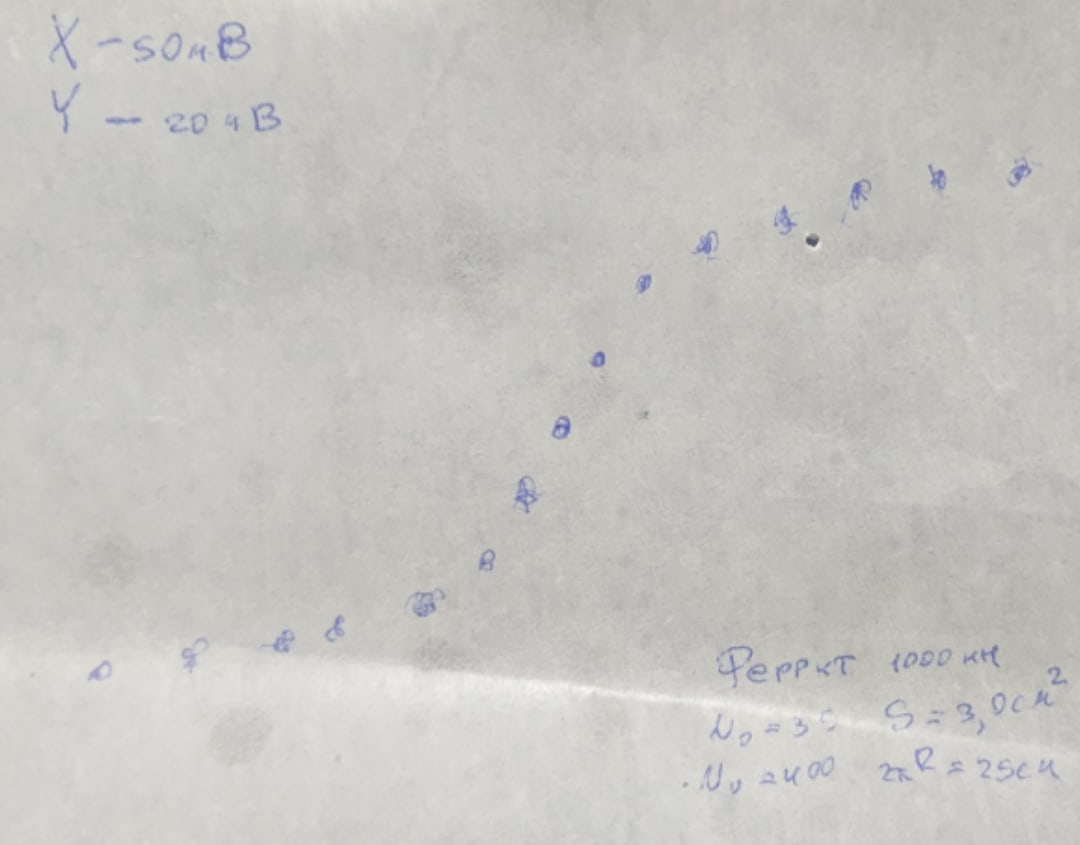
\includegraphics[width=0.8\textwidth]{fer.jpg}
    \label{fer}
\end{center}
\end{minipage}
\begin{minipage}{0.5\textwidth}
Из кривой намагничивания найдем значение дифференциальной магнитной пронициаемости:
    \begin{equation*}
        \frac{\mu_{diff}}{\mu_0} = \frac{1}{\mu_0}dB/dH = 6 \cdot 10^3
    \end{equation*}
И сравним с табличным:
    \begin{equation*}
        \frac{\mu_{diff \: tabular}}{\mu_0} = \frac{1}{\mu_0}dB/dH = 5 \cdot 10^3
    \end{equation*}
\end{minipage}

\subsection{Пермаллой}
\begin{minipage}{0.4\textwidth}
\begin{tabular}{|l|l|}
\hline
$N_0$ & 40        \\ \hline
$N_u$ & 200       \\ \hline
$S$   & 3.8см$^2$ \\ \hline
$2\pi R$ & 4см \\ \hline
\end{tabular}
\end{minipage}
\begin{minipage}{0.5\textwidth}
\begin{tabular}{|l|l|l|l|}
\hline
\multicolumn{2}{|l|}{X=20mV} & \multicolumn{2}{l|}{Y=50mV} \\ \hline
$[X_s]$:    & 5 дел.       & $250 \pm 18 $mA      &    $250 \pm 18$А/м  \\ \hline
$[Y_s]$:    & 2.8 дел.     & $140 \pm 3$ mV       &   $0.736 \pm 0.016$Тл   \\ \hline
$[X_c]$:    & 0.5 дел.     & $25.0 \pm 0.5$mA     &  $25.0 \pm 0.5$А/м    \\ \hline
$[Y_r]$:    & 1.6 дел.     & $80 \pm 3$mA         &  $0.42 \pm 0.02$Тл    \\ \hline
\end{tabular}
\end{minipage}\\

Измерим параметры предельной претли и пересчитаем значения B и H. Сравним их с табличными значениями.\\

\begin{minipage}{0.5\textwidth}
\begin{center}
    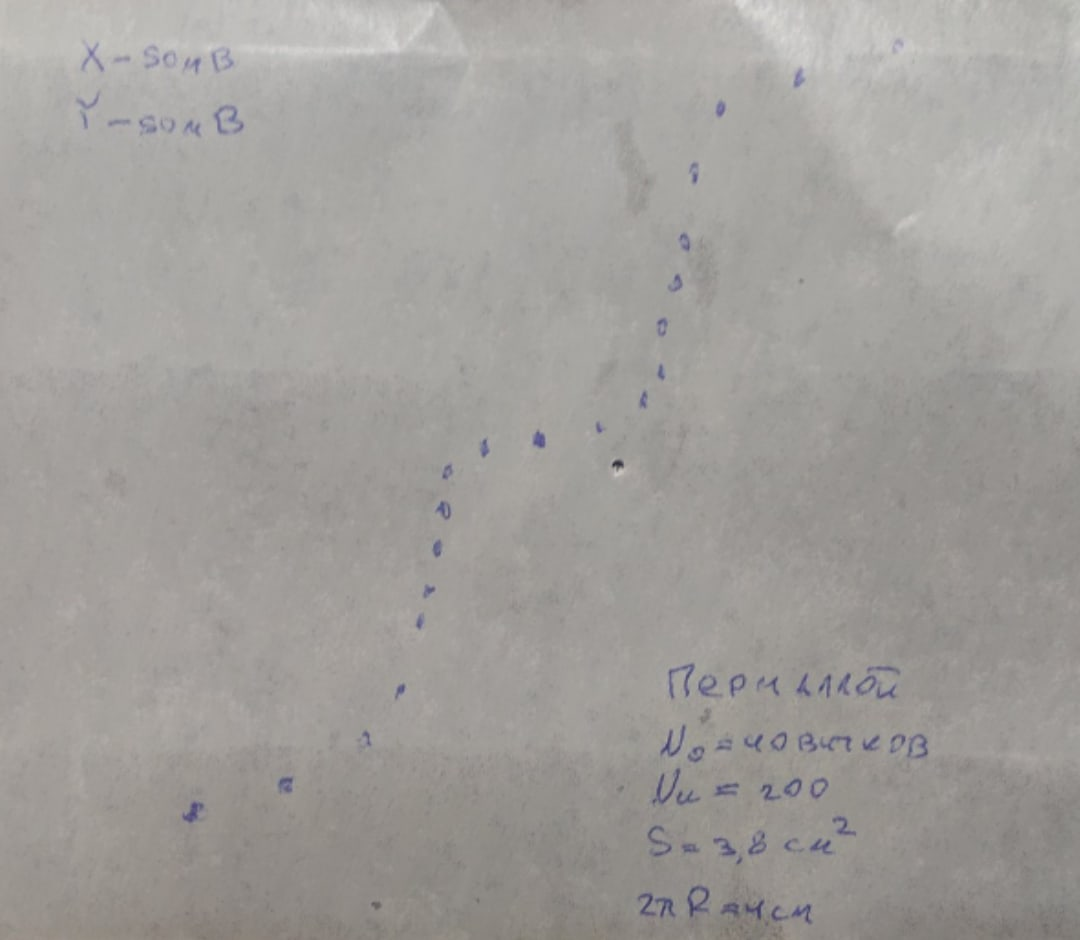
\includegraphics[width=0.8\textwidth]{perm.jpg}
    \label{fer}
\end{center}
\end{minipage}
\begin{minipage}{0.5\textwidth}
Из кривой намагничивания найдем значение дифференциальной магнитной пронициаемости:
    \begin{equation*}
        \frac{\mu_{diff}}{\mu_0} = \frac{1}{\mu_0}dB/dH = 1.6 \cdot 10^2
    \end{equation*}
И сравним с табличным:
    \begin{equation*}
        \frac{\mu_{diff \: tabular}}{\mu_0} = \frac{1}{\mu_0}dB/dH = 10^4
    \end{equation*}
\end{minipage}

\subsection{Кремнистое железо}
\begin{minipage}{0.4\textwidth}
\begin{tabular}{|l|l|}
\hline
$N_0$ & 35        \\ \hline
$N_u$ & 350       \\ \hline
$S$   & 1.2см$^2$ \\ \hline
$2\pi R$ & 10см \\ \hline
\end{tabular}
\end{minipage}
\begin{minipage}{0.5\textwidth}
\begin{tabular}{|l|l|l|l|}
\hline
\multicolumn{2}{|l|}{X=100mV} & \multicolumn{2}{l|}{Y=50mV} \\ \hline
$[X_s]$:    & 4.25 дел.    & $(107  \pm 3)\cdot 10 $mA      &    $(37 \pm 1)\cdot 10$А/м  \\ \hline
$[Y_s]$:    & 3 дел.    & $150 \pm 3$ mV        &   $1.43 \pm 0.03$Тл   \\ \hline
$[X_c]$:    & 0.5 дел.  &    $126 \pm 25$mA                  &   $44 \pm 9$А/м   \\ \hline
$[Y_r]$:    & 1.9 дел.  & $95 \pm 3$ mV                     &  $0.91 \pm 0.03$Тл     \\ \hline
\end{tabular}
\end{minipage}\\

Измерим параметры предельной претли и пересчитаем значения B и H. Сравним их с табличными значениями.\\

\begin{minipage}{0.5\textwidth}
\begin{center}
    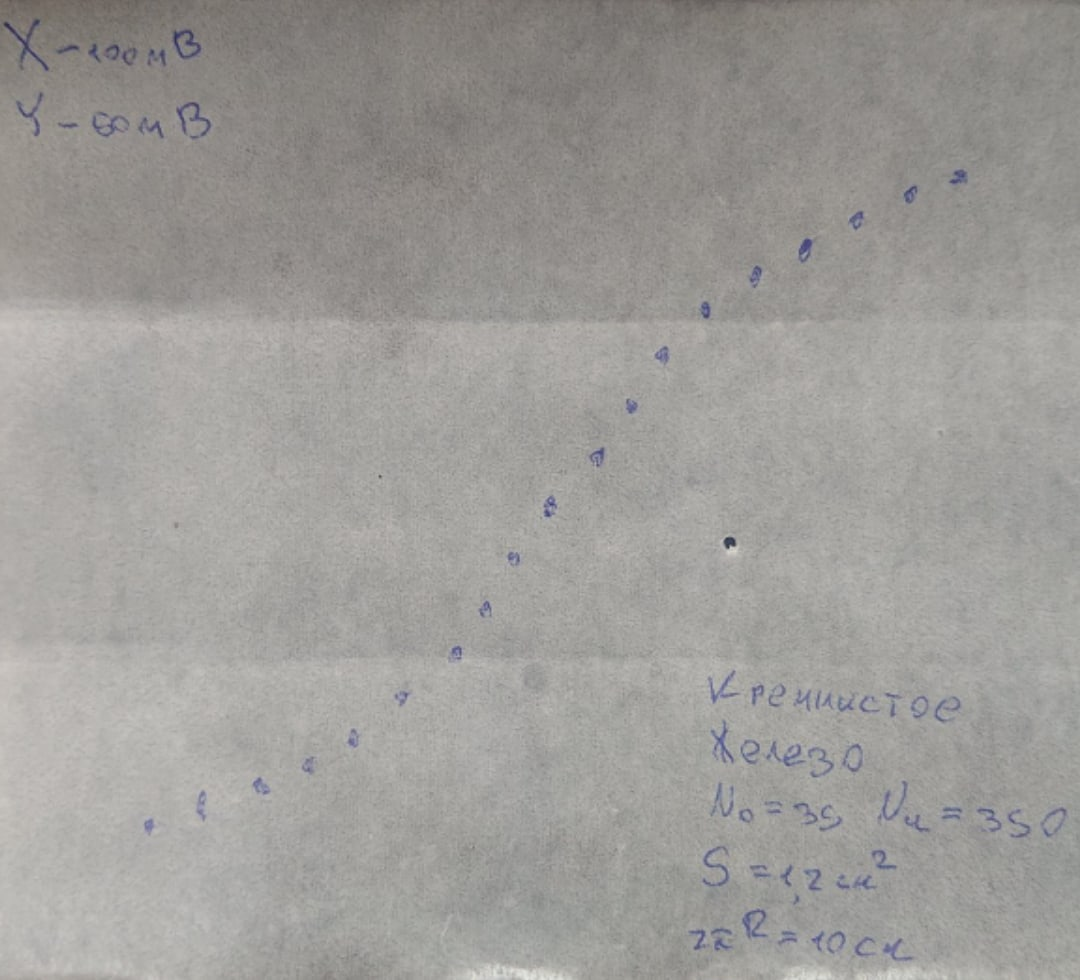
\includegraphics[width=0.8\textwidth]{iron.jpg}
    \label{fer}
\end{center}
\end{minipage}
\begin{minipage}{0.5\textwidth}
Из кривой намагничивания найдем значение дифференциальной магнитной пронициаемости:
    \begin{equation*}
        \frac{\mu_{diff}}{\mu_0} = \frac{1}{\mu_0}dB/dH = 6.7 \cdot 10^3
    \end{equation*}
И сравним с табличным:
    \begin{equation*}
        \frac{\mu_{diff \: tabular}}{\mu_0} = \frac{1}{\mu_0}dB/dH = 5.6 \cdot 10^3
    \end{equation*}
\end{minipage}

Проверим пременимость интегрирующей цепочки:
\begin{equation*}
    RC\Omega = \frac{U_{in}}{U_{out}} \approx 20 \gg 1
\end{equation*}
, значит цепочка применима. 

\section{Выводы}
Для двух \textit{(феррит и кремнистое железо)} из трех образцов мы получили результаты близкие к теоретическим. Отклонение от табличных значений сложно объяснить одной погрешностью измерений, так что, вероятно, большой вклад в отклонение внес тот факт, что сам момент, когда петля становится предельной, опередлить сложно. Для третьего образца значения получились значительно отличающиеся от теоретических, что, скорее всего, является следствием неправильно записанного диапазона измерений оциллографа или параметров образца.
\end{document}
